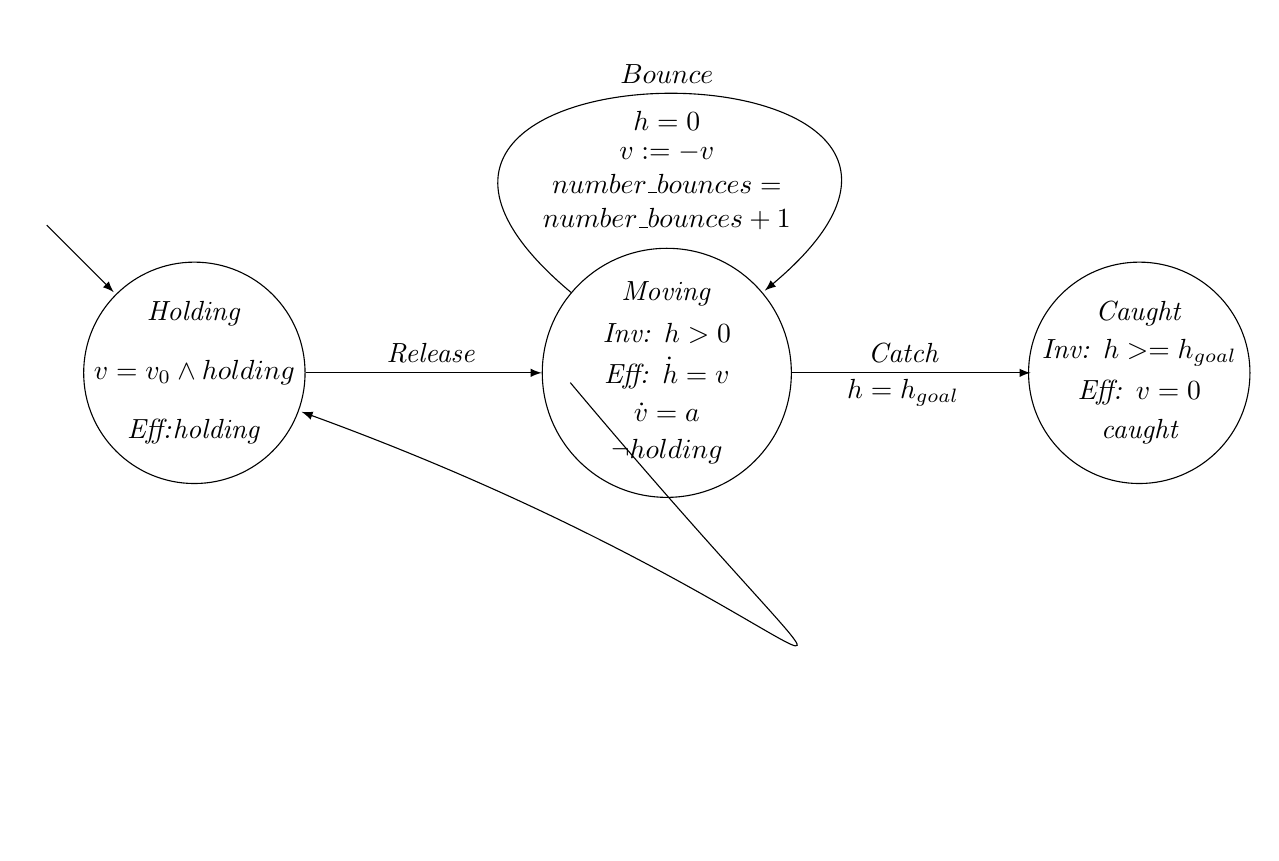
\begin{tikzpicture}[>=latex]
  \begin{scope}

%   \draw  (1,1) rectangle (7,1.5);

%\filldraw[black] (0,0) circle (2pt) node[anchor=west] {s};
\node (p1) at (-6,0.0) {};
\node (p2) at (-1.33,0.0) {};
\node (p3) at (4.745,0.0) {};




\node[circle, inner sep=4pt,draw, minimum height=80pt] (p1) at (-6,0) {};
\node (p4) at (-8,2.0) {};

\draw[->,shorten >=1pt] (p4) to  (p1);
\node (p0_d) at (-6.0,0.75) {\textit{Holding}};
%\node (p0_d) at (-6.0,0.25) {\textit{Inv:}   $h=h_0$};
\node (p0_d) at (-6.0,0){$v=v_0 \wedge holding $};
\node (p0_d) at (-6.0,-0.75) {\textit{Eff:}\textit{holding}};
\node (p0_d) at (-3.0,0.25) {$\textit{Release}$};
\draw[->,shorten >=1pt] (p2) to [out=310,in=340,loop,looseness=5.5] (p1);
\node (p0_d) at (-3.0,-0.25) {};

\node[circle, inner sep=4pt,draw, minimum height=90pt] (p2) at (0,0) {};
\draw[->] (p1) edge (p2);

\node (p1_d) at (0.0,1.0) {\textit{Moving}};
\node (p1_d) at (0.0,0.5) {\textit{Inv:} $h>0$};
\node (p1_d) at (0.0,0.0) {\textit{Eff:}  $\dot{h}=v$};
\node (p1_d) at (0.0,-0.5) {$\dot{v}=a$};
\node (p1_d) at (0.0,-1.0) {$\neg holding$};
\draw[->] (p2) edge (p3);
\node (p1_d) at (3.0,0.25) {$\textit{Catch}$};
\node (p1_d) at (3.0,-0.25) {$h=h_{goal}$};
\draw[->,shorten >=1pt] (p2) to [out=140,in=40,loop,looseness=5.5] (p2);
\node (p1_d) at (0.0, 3.2) {$h=0$};
\node (p1_d) at (0.0, 2.8) {$v:=-v$};
\node (p1_d) at (0.0, 2.4) {$number\_bounces = $};
\node (p1_d) at (0.0, 1.95) {$number\_bounces + 1 $};
\node (p1_d) at (0.0, 3.8) {$Bounce$};

\node[circle, inner sep=4pt,draw, minimum height=80pt] (p3) at (6,0) {};
\node (p2_d) at (6.0,0.75) {\textit{Caught}};
\node (p2_d) at (6.0,0.25) {\textit{Inv:}   $h>=h_{goal}$};
\node (p2_d) at (6.0,-0.25){\textit{Eff:}  $v=0$};
\node (p2_d) at (6.0,-0.75) {$\textit{caught}$};
\end{scope}
\end{tikzpicture}